\section{Diameter\-Ellipse Class Reference}
\label{classDiameterEllipse}\index{DiameterEllipse@{DiameterEllipse}}
{\tt \#include $<$diameterellipse.h$>$}

Inheritance diagram for Diameter\-Ellipse::\begin{figure}[H]
\begin{center}
\leavevmode
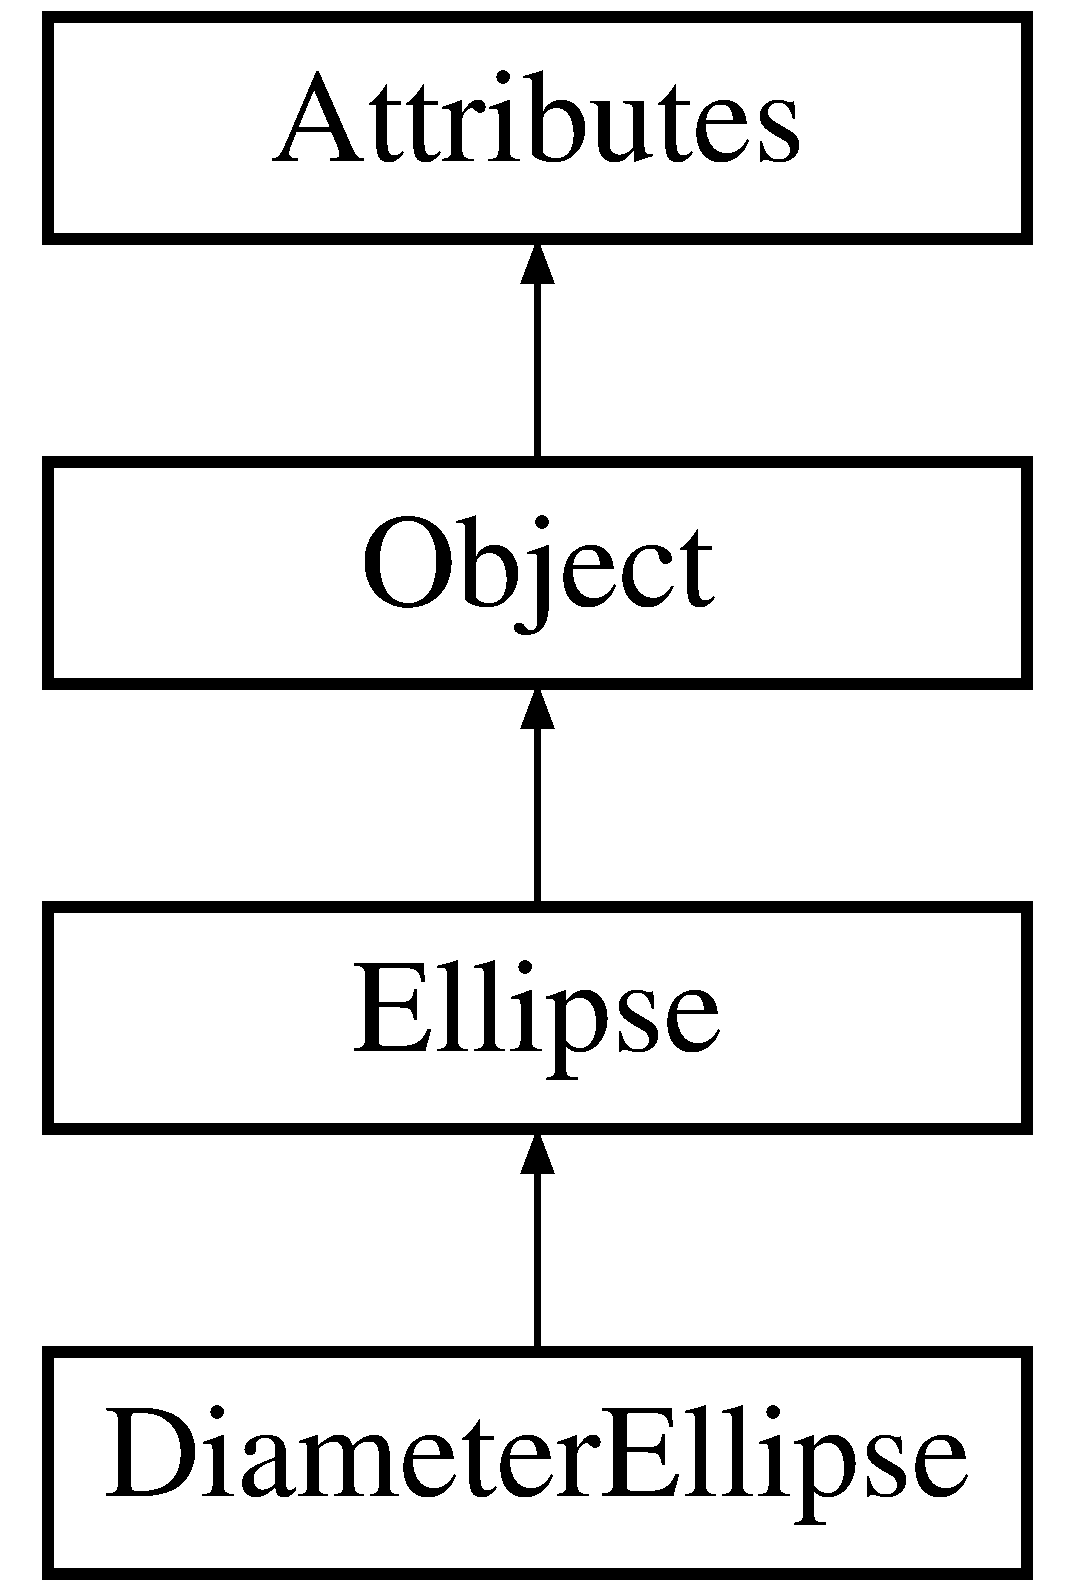
\includegraphics[height=4cm]{classDiameterEllipse}
\end{center}
\end{figure}
\subsection*{Public Methods}
\begin{CompactItemize}
\item 
{\bf Diameter\-Ellipse} ()
\item 
{\bf Diameter\-Ellipse} ({\bf Coordinate} $\ast$, {\bf Coordinate} $\ast$)
\item 
{\bf $\sim$Diameter\-Ellipse} ()
\end{CompactItemize}


\subsection{Detailed Description}
This class handles ellipses defined by their bounding box. This class is derived from {\bf Ellipse} {\rm (p.\,\pageref{classEllipse})}. \begin{Desc}
\item[Author: ]\par
Anthony Liekens \end{Desc}




\subsection{Constructor \& Destructor Documentation}
\index{DiameterEllipse@{Diameter\-Ellipse}!DiameterEllipse@{DiameterEllipse}}
\index{DiameterEllipse@{DiameterEllipse}!DiameterEllipse@{Diameter\-Ellipse}}
\subsubsection{\setlength{\rightskip}{0pt plus 5cm}Diameter\-Ellipse::Diameter\-Ellipse ()}\label{classDiameterEllipse_a0}


\index{DiameterEllipse@{Diameter\-Ellipse}!DiameterEllipse@{DiameterEllipse}}
\index{DiameterEllipse@{DiameterEllipse}!DiameterEllipse@{Diameter\-Ellipse}}
\subsubsection{\setlength{\rightskip}{0pt plus 5cm}Diameter\-Ellipse::Diameter\-Ellipse ({\bf Coordinate} $\ast$, {\bf Coordinate} $\ast$)}\label{classDiameterEllipse_a1}


\index{DiameterEllipse@{Diameter\-Ellipse}!~DiameterEllipse@{$\sim$DiameterEllipse}}
\index{~DiameterEllipse@{$\sim$DiameterEllipse}!DiameterEllipse@{Diameter\-Ellipse}}
\subsubsection{\setlength{\rightskip}{0pt plus 5cm}Diameter\-Ellipse::$\sim$Diameter\-Ellipse ()}\label{classDiameterEllipse_a2}




The documentation for this class was generated from the following files:\begin{CompactItemize}
\item 
{\bf diameterellipse.h}\item 
{\bf diameterellipse.cpp}\end{CompactItemize}
